\documentclass[12pt,a4paper]{report}

% ================= PACKAGES =================
\usepackage[utf8]{inputenc}
\usepackage[T1]{fontenc}
\usepackage[a4paper,margin=2.5cm,headheight=45pt]{geometry}
\usepackage{graphicx}
\usepackage{times}
\usepackage{indentfirst}
\usepackage{xcolor}
\usepackage{booktabs}
\usepackage{array}
\usepackage{multirow}
\usepackage{longtable}
\usepackage{amsmath}
\usepackage{listings}
\usepackage{fancyhdr}
\usepackage{titlesec}
\usepackage{tocloft}
\usepackage{caption}
\usepackage{float}
\usepackage{enumitem}
\usepackage{setspace}
\usepackage{xurl}
\usepackage{hyperref}

% ================= TOC / LIST OF FIGURES LEADER STYLE =================
\renewcommand{\cftchapleader}{\cftdotfill{\cftdotsep}}
\renewcommand{\cftsecleader}{\cftdotfill{\cftdotsep}}
\renewcommand{\cftsubsecleader}{\cftdotfill{\cftdotsep}}

% ================= HYPERLINK STYLE =================
\hypersetup{
    colorlinks=true,
    linkcolor=black,
    citecolor=black,
    urlcolor=blue,
    pdftitle={PerTrack -- Performance and OKR Management Platform},
}

% ================= PAGE STYLE =================
\pagestyle{fancy}
\fancyhf{}
\fancyhead[L]{
\includegraphics[height=0.9cm]{Images/Esprit.png}}
\fancyhead[R]{
\includegraphics[height=0.9cm]{Images/biatIt.jpg}}
\fancyfoot[R]{/ \thepage}
\renewcommand{\headrulewidth}{0pt}

% ================= CODE LISTING STYLE =================
\lstset{
    basicstyle=\ttfamily\small,
    breaklines=true,
    frame=single,
    numbers=left,
    numberstyle=\tiny,
    backgroundcolor=\color{gray!5},
    keywordstyle=\color{blue},
    commentstyle=\color{gray},
    stringstyle=\color{teal},
}

% ================= PLACEHOLDER MARKER =================
% Use \fillin{...} everywhere a fact is only known to the student
% (host institution identity, team methodology/tools actually used,
% real sprint dates, personal reflections). This renders clearly in
% the compiled PDF so nothing invented slips through unnoticed.
\newcommand{\fillin}[1]{\textcolor{red}{\textbf{[FILL IN: #1]}}}

% ================= FIGURE PLACEHOLDER =================
% None of the .drawio diagrams have been exported to PNG/PDF yet.
% This macro renders a clearly-marked placeholder box; once a diagram
% is exported into figures/<name>.png, replace the call with a plain
% \includegraphics figure using the same caption/label.
\newcommand{\figplaceholder}[3]{%
\begin{figure}[H]
\centering
\fbox{\parbox{0.85\textwidth}{\centering\vspace{1.4cm}\textbf{[PLACEHOLDER FIGURE]}\\[0.3em]Export \texttt{#1} to PNG/PDF and place in \texttt{figures/}\vspace{1.4cm}}}
\caption{#2}
\label{#3}
\end{figure}}

% ================= HEADER / COVER LOGOS =================
% ESPRIT (academic institution) and BIAT-IT (host company) logos, used
% in the running page header and on the title page.

% ================= DIAGRAM FIGURE =================
% Renders an already-exported diagram PNG (documentation/uml/generated/*.drawio
% -> Images/diagrams/*.png). #1=filename (no extension) #2=width (fraction of
% \textwidth) #3=caption #4=label
\newcommand{\diagramfig}[4]{%
\begin{figure}[H]
\centering
\includegraphics[width=#2\textwidth]{Images/diagrams/#1.png}
\caption{#3}
\label{#4}
\end{figure}}

% ================= SCREENSHOT PLACEHOLDER =================
% The only placeholder category left in the final report: a real screenshot
% of the running application, which cannot be captured here. #1=screen/action
% to capture #2=label
\newcommand{\screenshotplaceholder}[2]{%
\begin{figure}[H]
\centering
\fbox{\parbox{0.85\textwidth}{\centering\vspace{1.2cm}\textbf{[SCREENSHOT PLACEHOLDER]}\\[0.4em]Insert a screenshot of: #1\vspace{1.2cm}}}
\caption{#1}
\label{#2}
\end{figure}}
\definecolor{reportred}{RGB}{165,28,28}

\setstretch{1.15}
\tolerance=1
\emergencystretch=\maxdimen
\hyphenpenalty=10000
\hbadness=10000

\begin{document}

% ================= TITLE PAGE =================
\begin{titlepage}
    \centering
    \vspace*{0.5cm}

    
\includegraphics[height=2.2cm]{Images/Esprit.png}\par
    \vspace{1cm}

    \colorbox{reportred}{\parbox{0.85\textwidth}{\centering\color{white}\Large\bfseries\vspace{0.2cm} National Engineering Degree \vspace{0.2cm}}}\par
    \vspace{0.6cm}

    {\large \fillin{Academic year, e.g. 2025/2026}}\par
    \vspace{0.2cm}
    {\large SPECIALITY: INFORMATION TECHNOLOGY}\par
    \vspace{2cm}

    {\Huge \bfseries PerTrack: An Enterprise Performance\\[0.3em] and OKR Management Platform}\par
    \vspace{2cm}

    {\large By: \fillin{Student full name}}\par
    \vspace{1.5cm}

    {\large Supervised by:}\par
    \vspace{0.5cm}
    {\large Academic supervisor: \fillin{Name}}\par
    \vspace{0.3cm}
    {\large Corporate internship supervisor: \fillin{Name}}\par

    \vfill

    {\large BIAT-IT}\par
    \vspace{0.4cm}
    
\includegraphics[height=1.8cm]{Images/biatIt.jpg}\par
    \vspace{0.6cm}
    {\large \fillin{Submission date}}\par

\end{titlepage}

% ================= FRONT MATTER: ACKNOWLEDGEMENTS =================
\clearpage
\pagenumbering{gobble}
\fancyhf{}

\begin{center}
    \huge \textbf{Acknowledgements}
\end{center}
\vspace{1cm}
\fillin{Personal acknowledgements to the academic supervisor, the corporate internship supervisor, colleagues at BIAT-IT, professors, and family. Left as a placeholder since it can only be written by the student in their own words.}

\clearpage

% ================= TABLE OF CONTENTS =================
% Rendered with a plain centered chapter style (not the display-style
% divider used for real chapters below), so the TOC/LOF pages themselves
% stay compact instead of becoming full-page dividers.
{
\titleformat{\chapter}{\normalfont\Large\bfseries\centering}{}{0pt}{}
\titlespacing*{\chapter}{0pt}{0pt}{20pt}
\tableofcontents
\clearpage
\listoffigures
}
\clearpage

% ================= RESUME NUMBERED, HEADED PAGES =================
\pagestyle{fancy}
\fancyhf{}
\fancyhead[L]{
\includegraphics[height=0.9cm]{Images/Esprit.png}}
\fancyhead[R]{
\includegraphics[height=0.9cm]{Images/biatIt.jpg}}
\fancyfoot[R]{/ \thepage}
\pagenumbering{arabic}

% ================= CHAPTER DIVIDER STYLE =================
% Every \chapter (and \chapter*) below renders as its own centered,
% vertically-filled divider page, mirroring the per-chapter cover-page
% look of the reference report, before the section content resumes on
% a fresh page.
\titleformat{\chapter}[display]
  {\vspace*{\fill}\centering\normalfont\huge\bfseries}
  {\Large\scshape Chapter \thechapter}
  {20pt}
  {\Huge}
  [\vspace*{\fill}\clearpage]
\titlespacing*{\chapter}{0pt}{0pt}{0pt}

% ================================================================
\chapter*{General presentation}
\addcontentsline{toc}{chapter}{General presentation}

As part of my graduation project, I contributed to the design and development of \textbf{PerTrack}, an enterprise performance-evaluation and Objectives-and-Key-Results (OKR) management platform. PerTrack was built to replace informal, spreadsheet-driven performance review practices with a structured, auditable digital workflow: employees set goals within a defined annual cycle, track their progress through periodic check-ins, receive mid-year and final evaluations blending self-assessment with manager scoring, and see evaluation outcomes translate into concrete human-resources decisions such as promotions, bonuses, or coaching plans. The platform additionally embeds artificial-intelligence features to assist users in drafting higher-quality objectives and reviews, and a separate predictive microservice that estimates performance ratings and promotion readiness ahead of the formal evaluation cycle.

This report is organized to walk through the project the way it was actually built: from the context and motivation behind it, through the requirements and architecture that shaped its design, to the successive development sprints that delivered its features, and finally the DevOps pipeline that carries it from a developer's machine to a running, monitored deployment.

The first chapter introduces the host institution, the workspace I operated in, and the working methods and tools adopted by the team. The second chapter steps back to assess the problem PerTrack was meant to solve and situates it against existing performance-management software already on the market. The third chapter turns to the concrete requirements gathered for the platform and the architectural decisions taken before any code was written. Chapters four through eight each cover one development sprint, presenting the functional and technical specifications behind a coherent slice of the system before describing how it was actually built. The report closes with a general conclusion reflecting on what was delivered and what remains open for future iterations of the platform.

\clearpage

% ================================================================
\chapter{Global context}
\label{ch:global-context}

\section{Introduction}

This first chapter introduces BIAT-IT, the host institution where this internship took place, together with the project workspace I operated in. It then presents PerTrack itself and the users it was built for, before closing with the development methodology and the tools the team relied on throughout the project.

\section{Project workspace}

\subsection{Host institution}

This internship was hosted by \textbf{BIAT-IT}, the information-technology entity of BIAT (Banque Internationale Arabe de Tunisie), one of Tunisia's leading banking groups. As the group's internal IT arm, BIAT-IT builds and maintains the software systems supporting BIAT's operations instead of developing products for sale to external clients, and a performance-management platform for the bank's own staff falls squarely within that mandate. This internal-only positioning is reflected directly in the codebase: user registration is restricted to a single corporate email domain, which would not make sense for a multi-tenant product sold to outside organizations but is exactly what an internal tool built for one company's own employees requires. \fillin{Add further first-hand detail here if relevant: the specific department or team within BIAT-IT that hosted the internship, its size, and any additional context on why this performance-management tool was commissioned at this particular time.}

\begin{figure}[H]
\centering

\includegraphics[width=0.4\textwidth]{Images/biatIt.jpg}
\caption{BIAT-IT logo}
\label{fig:logo-biatit}
\end{figure}

\subsection{The PerTrack platform}

PerTrack is a role-based web application that runs an organization's annual performance-review cycle end to end. Employees define measurable objectives at the start of a cycle, track their progress through periodic check-ins, and are evaluated twice, at a mid-year checkpoint and at the close of the cycle, through a combination of self-assessment and manager review. Each final evaluation produces a weighted score and a rating label that Human Resources can act on directly, recording a promotion, bonus, or coaching decision without leaving the platform. Around this cycle, PerTrack also provides a Kanban task board, 360-degree feedback, calendar-synced meetings, automated notifications, and two AI components: a drafting assistant and a predictive rating model that offers an early signal ahead of the formal review.

\subsection{PerTrack's audience}

PerTrack was built for internal use within a single organization, so its audience is defined by role rather than by customer segment. \textbf{Collaborators} set their own objectives, submit check-ins, and complete self-assessments. \textbf{Team Leaders} review and approve their team's objectives and handle the manager side of evaluations. \textbf{Human Resources} manages the cycle itself and records the decisions -- promotions, bonuses, coaching plans -- that follow from final evaluations. An \textbf{Admin} role manages user accounts, team structures, and system-wide settings, independently of any single cycle.

\fillin{Name the specific department or business unit that piloted or uses PerTrack, if applicable.}

\subsection{Development methodology}

The team followed Agile principles throughout the project, structured specifically around Kanban rather than time-boxed Scrum sprints, since it suited a small team pulling continuously from a shared backlog better than committing to fixed two-week iterations with dedicated ceremonies.

\subsubsection{Kanban definition}

Kanban is a method for visualizing and controlling a team's flow of work through a shared board rather than through fixed-length iterations. Work items are represented as cards that move across a small number of columns representing their state, typically to-do, in-progress, review, and done, giving continuous visibility into what is being worked on, what is queued next, and what is already finished. Rather than replacing however a team already organizes itself, Kanban is meant to complement that existing process: work is pulled onto the board as capacity allows instead of being assigned up front, which keeps the team from being overloaded and lets it adapt quickly whenever priorities shift.

\subsubsection{Task management (Kanban)}

Task tracking was kept directly inside GitHub Projects instead of a separate tool disconnected from the code. The board was organized into To Do, In Progress, Review, and Done columns, with each card linked back to its GitHub issue and, once work started, to the pull request implementing it, so a card's column always reflected the real state of the corresponding branch instead of needing to be updated by hand. The five ``sprints'' this report is organized around -- entity and access management, objective and cycle workflow, evaluation and HR decisions, AI features, and DevOps -- correspond to five successive feature groupings pulled through that board in turn, each considered complete once its cards were built, tested, and merged. Using the same Kanban model the platform itself implements for its own task board made the day-to-day workflow familiar to reason about from both sides of the project.

\screenshotplaceholder{The team's GitHub Projects Kanban board (To Do / In Progress / Review / Done columns)}{fig:github-projects-board}

\section{Used tools}

\subsection{GitHub}

Version control and hosting were handled entirely through GitHub. Feature work was developed on topic branches merged into a shared \texttt{develop} branch through pull requests, with \texttt{develop} periodically promoted to \texttt{main} once a feature grouping was stable, giving the project a clear separation between code still under active work and code considered release-ready.

\subsection{GitHub Projects}

The Kanban board itself was kept directly in GitHub Projects, linked to the repository's issues, so that a backlog item, its board column, and the pull request implementing it stayed connected without needing a separate task-tracking tool disconnected from the code.

\subsection{Visual Studio Code}

Visual Studio Code was the primary editor across both the Node.js/React codebase and the Python microservice, chosen for its integrated terminal and Git tooling and for the breadth of extensions available for both JavaScript and Python development within a single editor.

\section{Conclusion}

This chapter set the scene for the rest of the report: the institution PerTrack was built for, the four roles it serves, and the working methods that shaped how the team delivered it. Framing the platform through these four vantage points early on turned out to matter well beyond this introductory chapter: every requirement, screen, and access rule described later traces back to one of Collaborator, Team Leader, Human Resources, or Admin, so establishing them clearly here made the rest of the specification easier to reason about. The development methodology and tooling described above also set the rhythm the remaining chapters follow, with each one corresponding to a single sprint delivered in turn. With that context established, the next chapter turns to the problem PerTrack was meant to solve in more concrete terms, and to how existing performance-management software on the market falls short of addressing it.

\clearpage

% ================================================================
% Remaining chapters continue below in subsequent files/sections.
% Placeholder chapter stubs kept here only so the document compiles
% end-to-end while the rest of the report is being written.
% ================================================================

\chapter{Project assessment and planning}
\label{ch:assessment}

\section{Introduction}

Having introduced the environment PerTrack was built in, this chapter turns to the reasoning behind the project itself. It restates, in more concrete terms, the problems the platform set out to solve; it looks at how existing performance-management software on the market addresses -- or fails to address -- those same problems; and it closes with the schedule that governed the internship.

\section{Description of PerTrack}

From a planning perspective, PerTrack is best understood as a single shared workflow viewed through four different lenses. A Collaborator opens the platform to see their own objectives for the current cycle, the tasks derived from them, and any feedback or notifications addressed to them. A Team Leader sees the same objective structure but for their entire team at once, together with the queue of items awaiting their review: objectives pending approval, check-ins to validate, and evaluations to score. Human Resources operates above the level of any single team, with visibility over every cycle, every final evaluation, and the decisions that follow from them. An Admin, finally, does not interact with the performance cycle at all in the functional sense, but with the structural scaffolding underneath it: user accounts, team hierarchies, and system configuration. Designing around these four vantage points from the start made it possible to reuse the same underlying data model across very different screens, instead of building four separate applications that happened to share a database.

\section{Problem statements}

Before any design work began, the project was framed around six concrete problems that an ad hoc, spreadsheet-based performance process leaves unresolved:

\begin{itemize}
    \item The absence of a structured, auditable objective-setting and approval workflow that ties an individual's goals to a defined organizational cycle, instead of leaving them scattered across disconnected documents.
    \item The lack of a standardized method for turning a self-assessment and a manager's assessment into a single, comparable weighted score, which otherwise leaves final ratings open to inconsistent, ad hoc judgment calls.
    \item The disconnect between an evaluation's outcome and the human-resources actions that should follow from it -- a rating that never automatically informs a promotion, bonus, or coaching decision is a rating that adds administrative overhead without changing anything.
    \item The absence of AI-assisted drafting support, at a time when employees and managers alike often struggle to phrase specific, measurable objectives and constructive review text under time pressure.
    \item The need for a complete audit trail: because performance data feeds directly into compensation and promotion decisions, every material change to it needs to be attributable and reviewable after the fact.
    \item The need for a repeatable, automated delivery pipeline capable of pushing changes safely across multiple environments (development, QA, staging, production) instead of relying on manual deployment steps.
\end{itemize}

\section{Available solutions}

Several established products already address parts of the performance-management space. Reviewing them was useful less as a benchmarking exercise and more as a way of identifying which trade-offs PerTrack should deliberately make differently.

\subsection{Workday Performance Management}

Workday is a large, established enterprise Human Capital Management suite in which performance reviews are one module among many: payroll, recruiting, and workforce planning all live in the same platform. Its strength is exactly that breadth: performance data sits alongside every other HR record for an employee. That same breadth is also its weakness for an organization that does not need or want the rest of the suite: configuring Workday for a single use case like objective-setting and review is a heavyweight, consultant-driven undertaking, not something a small internal team can stand up and iterate on quickly.

\begin{figure}[H]
\centering

\includegraphics[width=0.3\textwidth]{Images/workday.png}
\caption{Workday logo}
\label{fig:logo-workday}
\end{figure}

\subsection{Lattice}

Lattice is built specifically around OKRs and continuous feedback, with a lighter, more modern interface aimed at mid-size companies instead of large enterprises. It handles the goal-setting and check-in loop well, and its feedback and one-on-one features are comparable in spirit to what PerTrack offers. Where it is comparatively weak is on the compliance and audit side: for an organization in a regulated industry where every change to compensation-relevant data needs to be traceable, Lattice's audit capabilities are not built with that level of scrutiny in mind.

\begin{figure}[H]
\centering

\includegraphics[width=0.25\textwidth]{Images/latice.png}
\caption{Lattice logo}
\label{fig:logo-lattice}
\end{figure}

\subsection{15Five}

15Five centers the whole product around a weekly check-in cadence between an employee and their manager, with performance reviews layered on top of that rhythm. It is strong at keeping day-to-day engagement high, but its approval workflows are comparatively shallow: there is no equivalent of a formal, multi-state objective approval pipeline with explicit revision requests, which is central to how PerTrack structures its own objective lifecycle.

\begin{figure}[H]
\centering

\includegraphics[width=0.25\textwidth]{Images/15Five.png}
\caption{15Five logo}
\label{fig:logo-15five}
\end{figure}

\section{Study of the existing}

\begin{table}[H]
\centering
\small
\begin{tabular}{@{}p{2.2cm}p{5.3cm}p{5.3cm}@{}}
\toprule
\textbf{Tool} & \textbf{Strengths} & \textbf{Limitations} \\
\midrule
Workday & Deep HRIS integration; mature, enterprise-grade & Heavyweight to configure; expensive; overkill for a single use case \\
Lattice & Strong OKR and continuous-feedback UX & Weak audit trail; not built for regulated-industry compliance needs \\
15Five & Excellent weekly check-in cadence and engagement & Shallow, informal approval workflow; no multi-state objective lifecycle \\
\bottomrule
\end{tabular}
\caption{Feature and limitation comparison of existing performance-management solutions}
\label{tab:competitor-comparison}
\end{table}

\section{Project scheduling}

\fillin{Replace with the actual internship timeline. State the real start and end dates and the duration allocated to each of the following phases, ideally alongside a Gantt chart: entity and access management, objective and cycle workflow, evaluation and HR decisions, AI features, and DevOps.}

\begin{figure}[H]
\centering
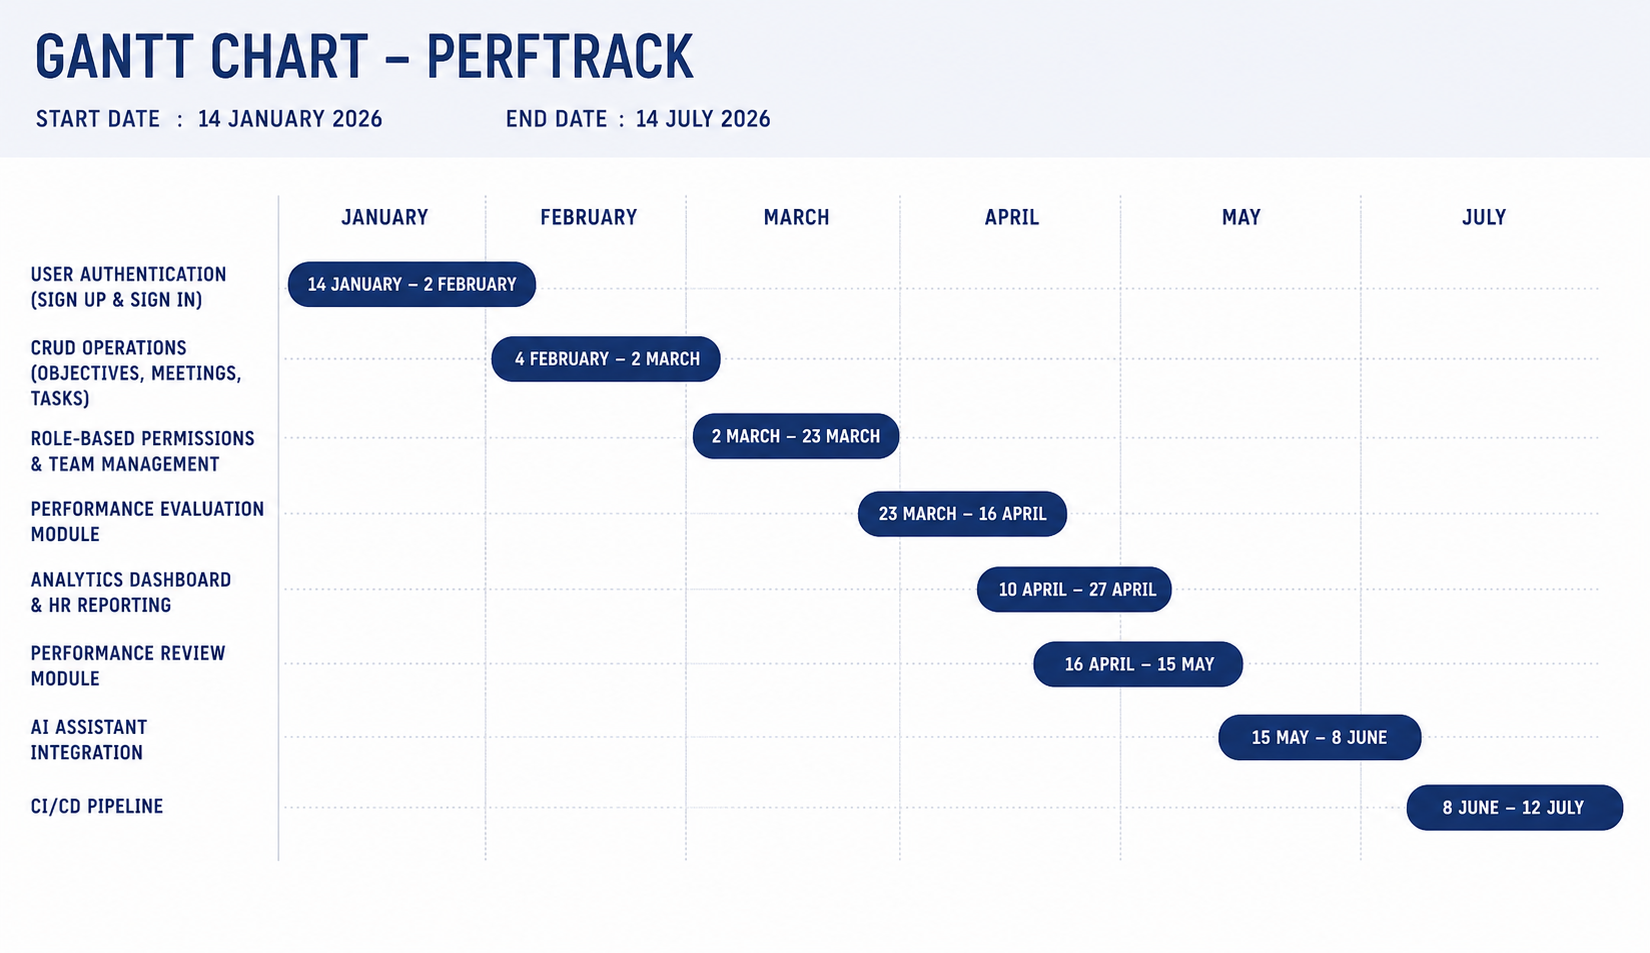
\includegraphics[width=\textwidth]{Images/Gant.png}
\caption{Project Gantt Chart}
\label{fig:gantt}
\end{figure}

\section{Conclusion}

This chapter has grounded the project in the concrete problems it was meant to solve and positioned it against the closest solutions already on the market. Reviewing Workday, Lattice, and 15Five side by side made one gap clear: no single existing product combines a formal, multi-state objective approval pipeline with the audit-trail rigor a platform feeding directly into compensation decisions eventually needs, which is precisely the space PerTrack was built to occupy. The next chapter moves from planning to specification: it lays out the functional and non-functional requirements gathered for PerTrack, the architecture chosen to satisfy them, and the technology stack used to implement that architecture.

\chapter{Project initiation}
\label{ch:initiation}

\section{Introduction}

With the problem clearly framed, this chapter turns to specification: who the platform serves and what each of them needs to be able to do, which quality attributes the system had to satisfy regardless of feature, the resulting backlog, the architecture chosen to support it, and the concrete technology stack used to build it.

\section{Requirements specification}

\subsection{Users identification}

Our platform is mainly intended for users with different roles, each interacting with the functionalities available on PerTrack based on a cumulative permission structure enforced at the middleware level: each role inherits everything the one below it can do, on top of its own additional powers. There are four roles:

\begin{itemize}
    \item \textbf{Collaborator:} creates and edits their own objectives while in draft state, submits check-ins, and completes self-assessments, scoped to resources they own.
    \item \textbf{Team Leader:} inherits everything a Collaborator can do, and additionally reviews, approves, rejects, or requests revisions on their team's objectives, scores check-ins, and performs the manager side of evaluations.
    \item \textbf{Human Resources:} inherits the Team Leader's permissions and adds cycle-level authority -- opening and closing cycles, finalizing evaluations across teams, and recording HR decisions and bonus or penalty entries.
    \item \textbf{Admin:} sits above all of them and bypasses ownership checks entirely, with authority over user accounts, team structures, and system-wide configuration such as access-control rules and notification templates.
\end{itemize}

\subsection{Functional requirements}

\subsubsection{User and team management}

The platform supports account authentication and role assignment, and organizes employees into teams. A team has exactly one leader and a list of members, but teams are not necessarily flat: a team may itself be nested under a parent team, so an organization's real departmental hierarchy (divisions containing departments containing individual teams) can be represented instead of forced into a single flat list.

\subsubsection{Cycle and objective management}

An annual performance cycle is divided into three phases -- goal-setting, mid-year review, and final evaluation -- each with its own start and end date. Within an open cycle, employees define objectives carrying a title, a description, a measurable success indicator, one or more key performance indicators, and a weight. Each objective then moves through a multi-state approval workflow: from draft, to submitted, to a manager's decision of approved, rejected, or revision-requested, through to locked once the goal-setting phase closes, and finally evaluated once the cycle concludes.

\subsubsection{Check-ins and progress tracking}

Once an objective is locked, the employee periodically submits check-ins recording their progress against it, optionally with supporting attachments. A team leader reviews each check-in and can approve it or send it back with a request for revision, creating a lightweight review loop that runs throughout the cycle and not only at its end.

\subsubsection{Task management}

Objectives can be broken down into individual tasks on a Kanban-style board, each carrying a status, a workflow stage, and optional time-tracking information. A task may be linked back to the objective it supports, so that day-to-day execution work remains traceable to the goal it serves, while still being manageable independently (reassigned, reprioritized, or rescheduled) without needing to touch the objective itself.

\subsubsection{Evaluation and HR decisions}

At the mid-year checkpoint, a lighter review takes place to catch drift early. At the close of the cycle, a full final evaluation combines the employee's self-assessment with the manager's score into a single weighted final score and a qualitative rating label. Human Resources reviews the resulting evaluations and can record a corresponding decision -- promotion, bonus, coaching, or other actions -- as well as standalone bonus or penalty entries tied to a given evaluation.

\subsubsection{Collaboration and communication}

Outside the formal cycle, employees and managers can exchange 360-degree feedback of several kinds -- praise, suggestion, concern, peer, or manager feedback -- optionally linked to a specific objective or meeting. Meetings can be scheduled directly on the platform, including two dedicated types for the mid-year and final evaluation conversations, and a user can connect an external Google or Outlook calendar account so that scheduled meetings sync automatically. A team-level activity feed surfaces recent activity to give a lightweight sense of what is happening across the team without needing to check each feature individually.

\subsubsection{Notifications and automated reminders}

The platform raises in-app notifications for a wide range of events -- an objective submitted or approved, a meeting invitation, a phase opening, an evaluation completed -- some triggered directly by user actions and others generated automatically by scheduled background jobs that watch for approaching deadlines and send reminders before they are missed.

\subsubsection{Correction requests}

Once an objective has been locked, its fields can no longer be edited directly, since doing so would undermine the integrity of a workflow that has already been approved. Instead, a user can submit a correction request specifying the field, its current value, and the proposed new value, which Human Resources or an Admin must explicitly approve or reject before the change is applied -- a deliberately narrower and more auditable path than reopening the objective for general editing.

\subsubsection{Reporting, analytics, and audit}

Final evaluations can be exported as PDF reports, and an analytics dashboard aggregates performance data across teams and cycles for Human Resources. Independently of both, every sensitive action taken on the platform -- who did what, to which record, and what changed -- is written to a permanent audit log, with its own reporting view for administrators.

\subsubsection{AI-assisted features}

Two AI capabilities support the core workflow without replacing it. A generative-AI assistant can suggest objective wording, key performance indicators, and draft review text on request. A separate, independent machine-learning service estimates a likely performance rating and promotion readiness from an employee's accumulated activity; it is meant to surface an early signal ahead of the formal evaluation, not to substitute for it.

\subsection{Non-functional requirements}

\subsubsection{Performance}

Requests are rate-limited to protect the platform under load, authenticated-user lookups are cached briefly to avoid repeated database round-trips on every request, and response payloads are compressed in transit.

\subsubsection{Security and auditability}

Given that PerTrack's data feeds directly into compensation and promotion decisions, security requirements go beyond simple authentication: role-based access control is enforced consistently across every endpoint, ownership checks prevent one user's data from being read or modified by another without the appropriate role, and every sensitive action is written to an immutable audit log.

\subsubsection{Observability}

Health-check endpoints and automated smoke tests confirm that a newly deployed version of the platform is actually serving traffic correctly before it is considered live, with more comprehensive infrastructure monitoring planned as a future addition.

\subsubsection{Evolvability}

The backend is organized so that routes, controllers, and models remain cleanly separated by domain, which keeps the addition of a new feature area (as happened repeatedly over the course of this project) from requiring changes scattered across unrelated parts of the codebase.

\subsection{Backlog}

{\small
\begin{longtable}{|>{\centering\arraybackslash}p{1.4cm}|p{3.0cm}|>{\centering\arraybackslash}p{1.0cm}|p{6.2cm}|>{\centering\arraybackslash}p{1.1cm}|}
\caption{High-level product backlog}\label{tab:backlog}\\
\hline
\textbf{Feature ID} & \textbf{Feature} & \textbf{Story Id} & \textbf{User Stories} & \textbf{Sprint} \\
\hline
\endfirsthead
\hline
\textbf{Feature ID} & \textbf{Feature} & \textbf{Story Id} & \textbf{User Stories} & \textbf{Sprint} \\
\hline
\endhead
\hline
\endfoot
\hline
\endlastfoot

\multirow{4}{*}{1} & \multirow{4}{3.0cm}{Entity and access management} & 1.1 & As a user, I can sign in and remain authenticated across requests without re-entering my credentials on every page. & 1 \\
\cline{3-5}
 & & 1.2 & As an Admin, I can create a user account and assign it a role. & 1 \\
\cline{3-5}
 & & 1.3 & As an Admin, I can create a team, assign its leader, and nest it under a parent team. & 1 \\
\cline{3-5}
 & & 1.4 & As HR, I can create a new performance cycle and open its first phase. & 1 \\
\hline
\multirow{6}{*}{2} & \multirow{6}{3.0cm}{Objective and cycle workflow} & 2.1 & As a Collaborator, I can create an objective with KPIs and a weight within an open cycle. & 2 \\
\cline{3-5}
 & & 2.2 & As a Team Leader, I can approve, reject, or request a revision on a submitted objective. & 2 \\
\cline{3-5}
 & & 2.3 & As a Collaborator, I can submit a check-in recording my progress on a locked objective. & 2 \\
\cline{3-5}
 & & 2.4 & As a Collaborator, I can manage my tasks on a Kanban board and link a task to an objective. & 2 \\
\cline{3-5}
 & & 2.5 & As a Collaborator, I can submit a correction request on a locked objective's field. & 2 \\
\cline{3-5}
 & & 2.6 & As a user, I receive a notification when an objective I own changes state or a deadline approaches. & 2 \\
\hline
\multirow{6}{*}{3} & \multirow{6}{3.0cm}{Evaluation, HR decisions and collaboration} & 3.1 & As a Collaborator, I can complete a self-assessment at the mid-year and final checkpoints. & 3 \\
\cline{3-5}
 & & 3.2 & As a Team Leader, I can score an employee's objectives and see the resulting weighted final score. & 3 \\
\cline{3-5}
 & & 3.3 & As HR, I can record a decision (promotion, bonus, coaching) against a final evaluation. & 3 \\
\cline{3-5}
 & & 3.4 & As a user, I can send and receive 360-degree feedback linked to an objective or meeting. & 3 \\
\cline{3-5}
 & & 3.5 & As a Team Leader, I can schedule a review meeting that syncs to my connected calendar. & 3 \\
\cline{3-5}
 & & 3.6 & As HR, I can export a final evaluation to PDF and view aggregate results on an analytics dashboard. & 3 \\
\hline
\multirow{3}{*}{4} & \multirow{3}{3.0cm}{AI features} & 4.1 & As a Collaborator, I can request an AI-suggested objective or set of KPIs while drafting a goal. & 4 \\
\cline{3-5}
 & & 4.2 & As a Team Leader, I can request an AI-drafted summary while writing a review. & 4 \\
\cline{3-5}
 & & 4.3 & As a Team Leader, I can view a predicted performance rating and promotion likelihood for an employee. & 4 \\
\hline
\multirow{3}{*}{5} & \multirow{3}{3.0cm}{DevOps} & 5.1 & As a developer, every push runs automated backend and frontend tests before anything is built. & 5 \\
\cline{3-5}
 & & 5.2 & As a developer, a passing pipeline automatically builds and pushes container images. & 5 \\
\cline{3-5}
 & & 5.3 & As an operator, a new image is automatically deployed to the target environment via GitOps. & 5 \\
\end{longtable}
}

\section{Project architecture}

\subsection{Logical architecture}

PerTrack follows a three-tier architecture with one addition that a purely three-tier system would not have: a presentation layer built with React, a treatment layer split between a Node.js/Express REST API and a separate Python/Flask microservice dedicated to machine-learning prediction, and a data layer backed by MongoDB. Splitting the treatment layer this way keeps the machine-learning code, and its very different dependency stack built around scikit-learn and XGBoost instead of JavaScript, isolated from the main application server. The trade-off is that the two services then need to be deployed and versioned independently.

\subsection{Platform structure}
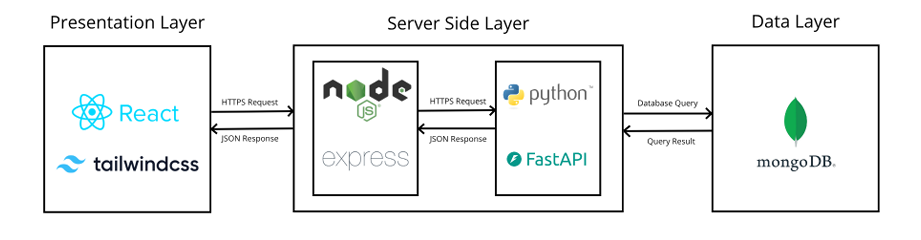
\includegraphics[width=0.25\textwidth]{Images/Project_Architecture.png}


The React frontend communicates with the Express backend exclusively over HTTPS, exchanging JSON payloads through a conventional request/response cycle. The Express backend, in turn, is the only component that talks directly to MongoDB, to the external generative-AI providers, and to the separate Flask prediction microservice; the frontend never calls the AI microservice directly. This gives the backend a single, consistent point at which to enforce authentication, authorization, rate-limiting, and audit logging before any request reaches a data source. The cost is that every AI-related feature depends on the main API server's availability even though the underlying computation happens elsewhere.

\diagramfig{20_api_communication_flow}{1.0}{API communication flow: from a React component through the API client layer to the Express middleware stack}{fig:api-flow}

\subsection{Backend architecture}

On the treatment layer's Express side, every request passes through a fixed middleware stack (Helmet, CORS, compression, JSON body parsing, XSS sanitization, Mongo-injection sanitization, and rate limiting) before it reaches any of the backend's twenty-six route modules. Authentication, role, and ownership checks are applied per-route on top of that shared stack instead of being folded into it, since not every route requires the same access rules.

\diagramfig{11_backend_architecture}{0.68}{Backend architecture: middleware stack, route modules, and the auth/role/ownership layer}{fig:backend-arch}

\subsection{Frontend architecture}

The frontend centralizes route, role, and cycle-phase metadata in a single \texttt{routeConfig.jsx} file, from which both the navigation sidebar and the route guards are generated. This avoids maintaining the sidebar and the routing table as two separately hand-maintained lists that could drift apart. \texttt{AuthContext} and \texttt{ActiveCycleContext} expose the current user and cycle state to any of the roughly two dozen lazy-loaded pages, while \texttt{RouteGuard}, \texttt{ProtectedRoute}, and \texttt{CyclePhaseRoute} enforce, respectively, authentication, role, and cycle-phase eligibility before a page is allowed to render.

\diagramfig{12_frontend_architecture}{0.55}{Frontend architecture: route configuration, guards, context providers, and pages}{fig:frontend-arch}

\subsection{Component diagram}

\diagramfig{14_component_diagram}{0.9}{Component diagram: Frontend SPA, Backend API (including the generative AI service), ML prediction microservice, and MongoDB}{fig:component}

\subsection{Package diagram}

Within the backend, code is organized into distinct packages by responsibility (routes, middleware, controllers, services, and utilities), so that a route module stays a thin definition of endpoints and the handlers, business logic, and cross-cutting concerns behind them live in clearly separated locations.

\diagramfig{15_package_diagram}{0.9}{Package diagram: backend module organization (routes, middleware, controllers, services, utils)}{fig:package}

\subsection{Data model (entity-relationship diagram)}

Although MongoDB does not enforce relational constraints, the domain still has clear reference relationships between collections: a Team references its leader and parent team, and an Objective references its owning User and Cycle. The following logical ERD makes these relationships explicit for readers more familiar with relational modeling.

\diagramfig{16_erd_logical}{1.0}{Logical entity-relationship diagram of the core collections, with references shown as FK-style associations}{fig:erd}

\section{Tools and technologies}

\subsection{Node.js}
Node.js provides the JavaScript runtime the backend is built on, chosen for its non-blocking I/O model, which suits an API server handling many concurrent, mostly I/O-bound requests (database queries, calls to external AI providers) instead of heavy CPU-bound computation.

\begin{figure}[H]
\centering

\includegraphics[width=0.2\textwidth]{Images/Nodejs.png}
\caption{Node.js logo}
\label{fig:logo-nodejs}
\end{figure}

\subsection{Express.js}
Express.js is the web framework layered on top of Node.js, providing the routing, middleware chain, and request/response abstractions the backend's twenty-six route modules are built around.

\begin{figure}[H]
\centering

\includegraphics[width=0.2\textwidth]{Images/express.png}
\caption{Express.js logo}
\label{fig:logo-express}
\end{figure}

\subsection{MongoDB / Mongoose}
MongoDB is the document database underlying the platform, chosen for the flexibility its schema-less documents give to the many sub-document structures the domain requires -- an objective's KPIs, comments, attachments, and activity log all live as embedded arrays within a single objective document. Mongoose provides the schema definition, validation, and query layer used to interact with it from Node.js.

\begin{figure}[H]
\centering

\includegraphics[width=0.2\textwidth]{Images/mongodb.png}
\caption{MongoDB logo}
\label{fig:logo-mongodb}
\end{figure}

\subsection{React}
React is the library the frontend is built with, chosen for its component model and the ecosystem of supporting libraries around it.

\begin{figure}[H]
\centering

\includegraphics[width=0.25\textwidth]{Images/react.png}
\caption{React logo}
\label{fig:logo-react}
\end{figure}

\subsection{Vite}
Vite is the build tool and development server used alongside React, valued for its fast start-up and hot-reload times during development compared to older bundler-based tooling.

\begin{figure}[H]
\centering
\centering

\includegraphics[width=0.25\textwidth]{Images/vite.png}
\caption{Vite logo}
\label{fig:logo-vite}
\end{figure}

\subsection{Python / Flask}
Python, via the Flask micro-framework, powers the standalone machine-learning prediction service. Python was the natural choice here specifically because the machine-learning ecosystem it gives access to (scikit-learn and XGBoost in this case) is far more mature than any equivalent available in JavaScript.

\begin{figure}[H]
\centering

\includegraphics[width=0.18\textwidth]{Images/python.png}
\caption{Python logo}
\label{fig:logo-python}
\end{figure}


\subsection{Docker}
Docker packages both the backend and frontend applications into portable, self-contained images, ensuring that the environment a container runs in during automated testing is the same one it runs in in production.

\begin{figure}[H]
\centering

\includegraphics[width=0.15\textwidth]{Images/docker.png}
\caption{Docker logo}
\label{fig:logo-docker-ch3}
\end{figure}

\subsection{Kubernetes}
Kubernetes orchestrates the deployed containers across development, QA, staging, and production environments.

\begin{figure}[H]
\centering

\includegraphics[width=0.25\textwidth]{Images/Kubernetes.png}
\caption{Kubernetes logo}
\label{fig:logo-k8s}
\end{figure}

\subsection{ArgoCD}
ArgoCD implements a GitOps delivery model on top of Kubernetes: the cluster's actual running state is continuously reconciled against what is declared in a Git repository, instead of being pushed to it imperatively.

\begin{figure}[H]
\centering

\includegraphics[width=0.25\textwidth]{Images/ArgoCD.png}
\caption{ArgoCD logo}
\label{fig:logo-argocd}
\end{figure}

\subsection{Postman}
Postman is used throughout development to design, execute, and validate API requests against the backend independently of the frontend, which is particularly useful for exercising endpoints (such as administrative or AI-related routes) that do not yet have a corresponding UI screen.

\begin{figure}[H]
\centering

\includegraphics[width=0.25\textwidth]{Images/postman.png}
\caption{Postman logo}
\label{fig:logo-postman}
\end{figure}

\subsection{@dnd-kit}
\texttt{@dnd-kit} is the drag-and-drop library used on the frontend to implement the Kanban task board, allowing a task to be dragged between status columns with the resulting state change persisted back to the API.

\begin{figure}[H]
\centering

\includegraphics[width=0.2\textwidth]{Images/dnd.png}
\caption{@dnd-kit logo}
\label{fig:logo-dndkit}
\end{figure}

\section{Conclusion}

This chapter has turned the problem framed in Chapter 2 into a concrete specification: the roles the system serves, the functional and non-functional requirements those roles impose, the architecture chosen to satisfy them, and the technologies used to implement it. Nothing in the backlog that follows was decided independently of this chapter's architecture: the three-tier split between presentation, treatment, and data layers, and the decision to isolate machine-learning prediction in its own Flask service, both directly shape how work was later divided across the five sprints. The next five chapters each take one slice of this specification and walk through it as a development sprint, from functional design through to the working feature it produced.

\chapter{Sprint 1: Entity and access management}
\label{ch:sprint1}

\section{Introduction}

This first sprint delivered the layer every other feature in the platform depends on: user accounts, team structures, annual cycles, and the role-based access control enforced on top of them. Nothing described in the following chapters (objectives, evaluations, AI assistance) can function without an authenticated user attached to a team within an open cycle. That is why this sprint was scheduled first instead of being treated as background infrastructure.

\section{Functionality overview}

By the end of this sprint, a user could sign in and receive a session that persisted securely across requests; an administrator could create user accounts, assign them a role, and organize them into teams, including teams nested under a parent team to reflect a real departmental hierarchy; and Human Resources could create a new annual cycle and open its first phase, making the platform ready to receive objectives.

\section{Functional specifications}

\subsection{Sprint backlog}

\begin{table}[H]
\centering
\small
\begin{tabular}{|>{\centering\arraybackslash}p{1.4cm}|p{5.3cm}|>{\centering\arraybackslash}p{1.3cm}|p{5.3cm}|}
\hline
\textbf{Story Id} & \textbf{User Stories} & \textbf{Task Id} & \textbf{Tasks} \\
\hline
\multirow{3}{*}{1.1} & \multirow{3}{5.3cm}{As a user, I can sign in and remain authenticated across requests without re-entering my credentials on every page.} & 1.1.1 & Implement JWT-based sign-in \\
\cline{3-4}
 & & 1.1.2 & Implement refresh-token rotation and session persistence \\
\cline{3-4}
 & & 1.1.3 & Build the sign-in page and route guards \\
\hline
\multirow{3}{*}{1.2} & \multirow{3}{5.3cm}{As an Admin, I can create a user account and assign it a role.} & 1.2.1 & Implement user creation endpoint with role assignment \\
\cline{3-4}
 & & 1.2.2 & Enforce role-based access control across routes \\
\cline{3-4}
 & & 1.2.3 & Build the admin user management screen \\
\hline
\multirow{3}{*}{1.3} & \multirow{3}{5.3cm}{As an Admin, I can create a team, assign its leader, and nest it under a parent team.} & 1.3.1 & Implement team creation with leader assignment \\
\cline{3-4}
 & & 1.3.2 & Implement parent-team nesting and hierarchy validation \\
\cline{3-4}
 & & 1.3.3 & Build the team management screen \\
\hline
\multirow{3}{*}{1.4} & \multirow{3}{5.3cm}{As HR, I can create a new performance cycle and open its first phase.} & 1.4.1 & Implement cycle creation endpoint \\
\cline{3-4}
 & & 1.4.2 & Implement phase transition logic \\
\cline{3-4}
 & & 1.4.3 & Build the cycle management screen \\
\hline
\end{tabular}
\caption{Sprint 1 backlog}
\label{tab:sprint1-backlog}
\end{table}

\subsection{Use case diagram}
\begin{figure}[H]
    \centering
    
\includegraphics[width=1.0\textwidth]{C:/Users/moata/Downloads/Use_case_general.jpg}
\end{figure}

\subsection{Sequence diagram}

\begin{figure}[H]
    \centering
    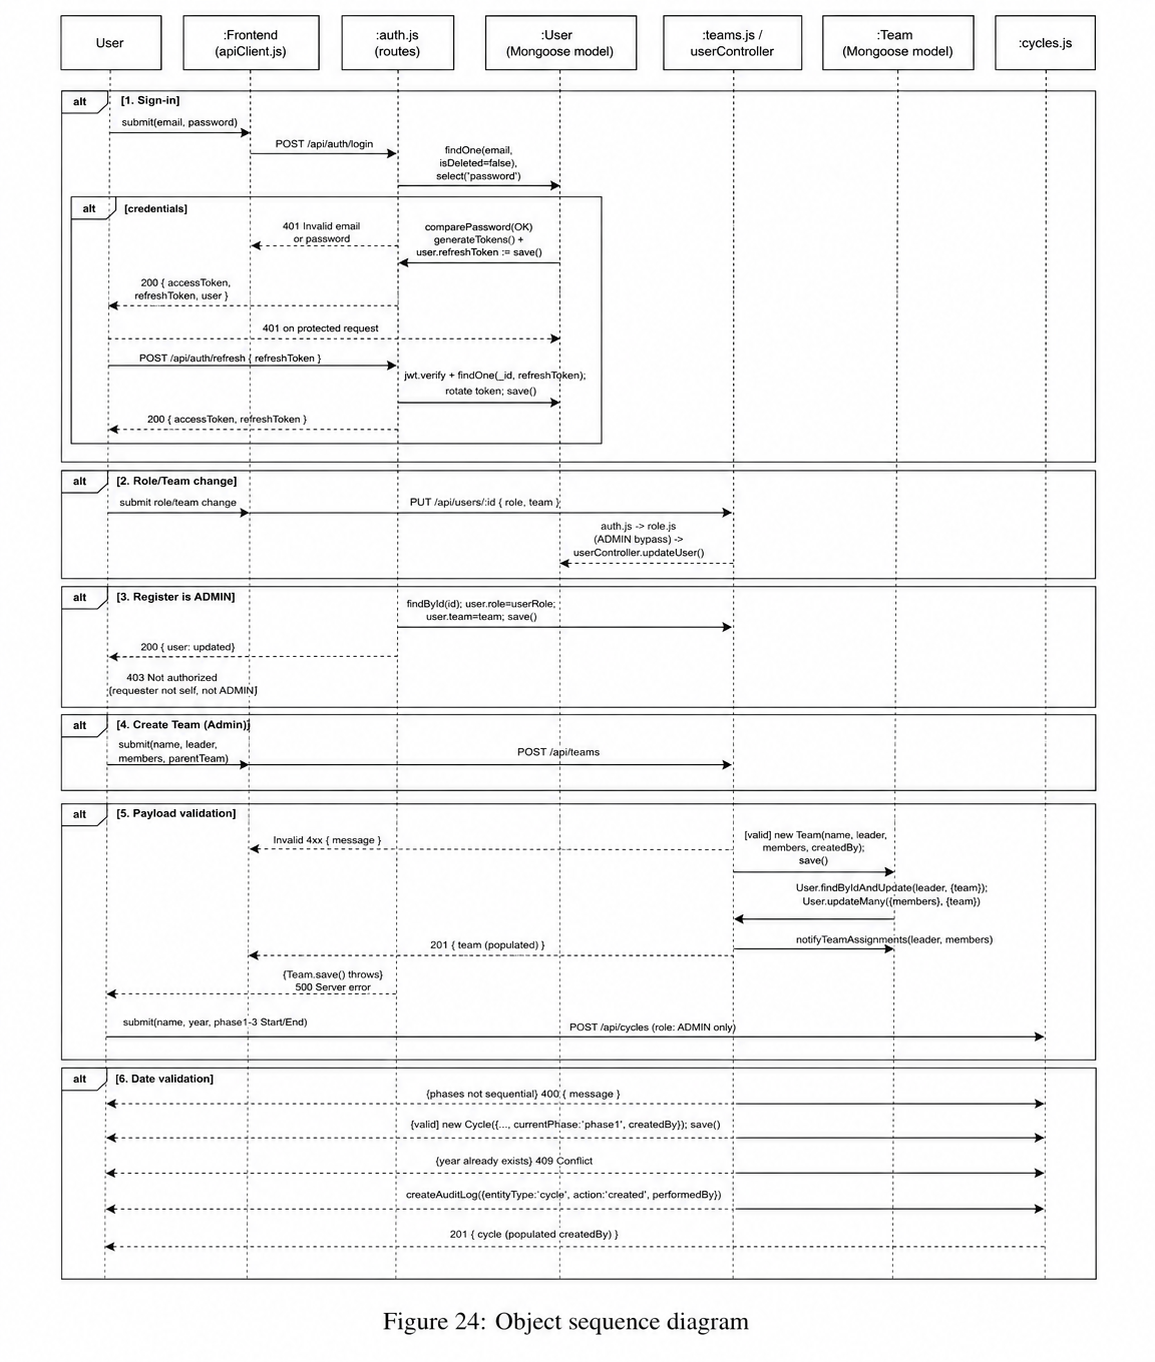
\includegraphics[width=1.0\textwidth]{Images/SEq.png}
    \caption{Sprint 1 sequence: sign-in and refresh-token rotation, admin user/role update, team creation, and cycle creation}
    \label{fig:seq-auth}
\end{figure}\subsection{Class/entity diagram}

\begin{figure}[H]
    \centering
    
\includegraphics[width=1.0\textwidth]{C:/Users/moata/Downloads/Diag_de_class.jpg}
    \caption{User, Team, and Cycle classes, including the Team self-reference used for sub-team nesting}
    \label{fig:class-entity}
\end{figure}


\section{Technical specifications}

\subsection{JSON Web Token (access and refresh)}

Authentication is implemented with a pair of JSON Web Tokens instead of a single long-lived token. A short-lived access token is issued on login and attached to every subsequent request as a bearer token; a longer-lived refresh token, stored server-side against the user's record, is used solely to obtain a new access token once the current one expires, without requiring the user to re-enter their credentials. This split keeps the token an attacker could steal from a compromised client short-lived, while the refresh token itself is checked against the stored value on every rotation.

\subsection{Bcrypt}

Passwords are never stored in plain text. Before a new user's password is persisted, it is hashed with bcrypt, a deliberately slow, salted hashing algorithm designed to resist brute-force attacks even if the underlying database is compromised. Login compares the submitted password against the stored hash using the same algorithm instead of attempting to reverse it.

\subsection{Role and ownership middleware (RBAC)}

Two middleware layers enforce access control on every protected route. The first checks the authenticated user's role against a list of roles allowed to reach a given endpoint, with the Admin role configured to bypass this check entirely. The second, applied to routes that operate on a specific resource, verifies that the authenticated user actually owns (or manages, in the case of a Team Leader acting on a team member's data) the resource being accessed, so that a Collaborator cannot read or modify another Collaborator's objectives simply by guessing an identifier.


\subsection{Audit logging}

Every action that touches sensitive data -- creating a user, changing a role, approving an objective, recording an HR decision -- is written to a permanent audit log entry capturing who performed the action, what it was, which record it affected, and a before/after snapshot of the change. This logging is implemented as a thin layer invoked from within the relevant controllers, not as a blanket, undiscriminating request logger, so that the audit trail stays focused on actions that actually matter for compliance review.

\section{Build phase}

\subsection{Sign-in and session flow}

The sign-in screen collects an email and password, submits them to the authentication endpoint, and on success stores the returned access token for use on subsequent requests while the refresh token is retained server-side. From that point on, every protected page checks the token's validity and the user's role before rendering, redirecting back to sign-in if either check fails.

\screenshotplaceholder{The sign-in screen (email/password form)}{fig:ss-signin}

\subsection{Team hierarchy management}

An administrator can create a team, assign it a leader, and optionally nest it under an existing parent team, building up a tree structure that mirrors the organization's real reporting lines. Each user also has access to a ``My Team'' view showing their team's roster and, where the team itself has sub-teams, a rolled-up view of those as well.

\screenshotplaceholder{The team creation form, showing leader/member assignment and parent-team selection}{fig:ss-team-mgmt}

\subsection{Cycle creation and phase configuration}

Human Resources creates a new cycle by giving it a name and a year, then defines the start and end dates of each of its three phases. Opening the first phase is what makes the cycle available for objective creation; the platform prevents two phases from overlapping and enforces that phases occur in sequence.

\screenshotplaceholder{The cycle management screen, showing the three-phase date configuration}{fig:ss-cycle-mgmt}

\section{Conclusion}

With authentication, roles, teams, and cycles in place, the platform had a foundation every subsequent sprint could build directly on top of. In practice this meant the JWT-based session handling, the role-and-ownership middleware, and the audit-logging layer built here were never revisited as separate concerns later on; every feature introduced afterward simply plugged into checks that already existed instead of reinventing them. The next chapter turns to the feature built on that foundation first, and arguably the most complex in the entire platform: the objective and cycle workflow itself.

\chapter{Sprint 2: Objective and cycle workflow}
\label{ch:sprint2}

\section{Introduction}

This sprint delivered what is, in both business importance and implementation complexity, the core of PerTrack: the objective lifecycle itself, together with the check-in loop, task board, correction-request workflow, and notification system that surround it. Where Sprint 1 built the scaffolding, this sprint is where the platform started doing the job it was actually built for.

\section{Functionality overview}

Within an open cycle, an employee can now create an objective with key performance indicators and a weight, submit it for review, and see it move through approval, rejection, or a request for revision at their team leader's hands. Once approved and the goal-setting phase closes, the objective locks and progress is tracked through periodic check-ins, with day-to-day work broken down further on a Kanban task board linked back to the objective it supports. A user who later needs to correct a locked objective's field can submit a correction request instead of editing it directly, and the whole workflow is threaded through with notifications that keep everyone informed as items move between states.

\section{Functional specifications}

\subsection{Sprint backlog}

\begin{table}[H]
\centering
\small
\begin{tabular}{|>{\centering\arraybackslash}p{1.4cm}|p{5.3cm}|>{\centering\arraybackslash}p{1.3cm}|p{5.3cm}|}
\hline
\textbf{Story Id} & \textbf{User Stories} & \textbf{Task Id} & \textbf{Tasks} \\
\hline
\multirow{3}{*}{2.1} & \multirow{3}{5.3cm}{As a Collaborator, I can create an objective with KPIs and a weight within an open cycle.} & 2.1.1 & Implement objective creation endpoint with embedded KPIs \\
\cline{3-4}
 & & 2.1.2 & Enforce open-cycle and weight validation rules \\
\cline{3-4}
 & & 2.1.3 & Build the objective creation form \\
\hline
\multirow{3}{*}{2.2} & \multirow{3}{5.3cm}{As a Team Leader, I can approve, reject, or request a revision on a submitted objective.} & 2.2.1 & Implement approval, rejection, and revision-request endpoints \\
\cline{3-4}
 & & 2.2.2 & Implement the objective state machine and locking on approval \\
\cline{3-4}
 & & 2.2.3 & Build the objective review screen \\
\hline
\multirow{3}{*}{2.3} & \multirow{3}{5.3cm}{As a Collaborator, I can submit a check-in recording my progress on a locked objective.} & 2.3.1 & Implement check-in submission endpoint \\
\cline{3-4}
 & & 2.3.2 & Link check-in history to objective progress tracking \\
\cline{3-4}
 & & 2.3.3 & Build the check-in submission form \\
\hline
\multirow{3}{*}{2.4} & \multirow{3}{5.3cm}{As a Collaborator, I can manage my tasks on a Kanban board and link a task to an objective.} & 2.4.1 & Implement task CRUD endpoints linked to an objective \\
\cline{3-4}
 & & 2.4.2 & Implement drag-and-drop status updates with @dnd-kit \\
\cline{3-4}
 & & 2.4.3 & Build the Kanban task board \\
\hline
\multirow{3}{*}{2.5} & \multirow{3}{5.3cm}{As a Collaborator, I can submit a correction request on a locked objective's field.} & 2.5.1 & Implement correction-request creation endpoint \\
\cline{3-4}
 & & 2.5.2 & Implement the correction-request approval workflow \\
\cline{3-4}
 & & 2.5.3 & Build the correction-request form \\
\hline
\multirow{3}{*}{2.6} & \multirow{3}{5.3cm}{As a user, I receive a notification when an objective I own changes state or a deadline approaches.} & 2.6.1 & Implement notifications on objective state changes \\
\cline{3-4}
 & & 2.6.2 & Implement deadline-based notification scheduling \\
\cline{3-4}
 & & 2.6.3 & Build the notification center UI \\
\hline
\end{tabular}
\caption{Sprint 2 backlog}
\label{tab:sprint2-backlog}
\end{table}

\subsection{Use case diagram}

\begin{figure}[H]
    \centering
    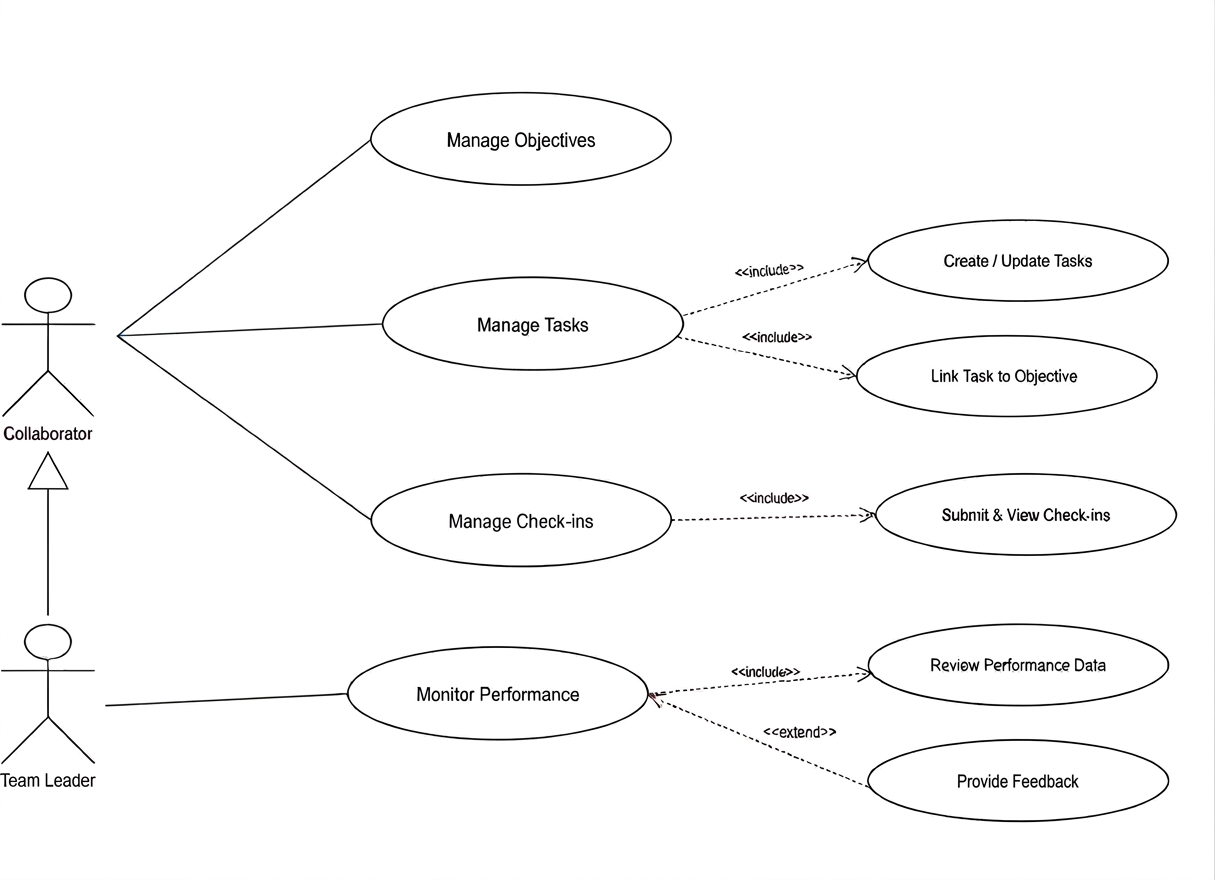
\includegraphics[width=0.95\textwidth]{Images/Diag_de_usecase_Sprint2.jpg}
    \caption{Use case diagram -- Sprint 2}
    \label{fig:usecase-sprint2}
\end{figure}

\subsection{Sequence diagram}

\diagramfig{22_objective_approval_sequence}{1.0}{Sprint 2 sequence: objective creation and approval, check-in submission and review, task management, and correction requests}{fig:seq-objective}

\subsection{Document/class model diagram}

\diagramfig{PerTrack_Document_Model_Diagram}{1.0}{Objective sub-document structure, Task, and CorrectionRequest}{fig:doc-objective}

\subsection{State machine diagram}

An objective's approval workflow is best understood as a state machine, not a simple flag: from Draft it moves to Submitted, then to PendingApproval, from which a Team Leader's decision branches it to Approved, Rejected, or back to Draft for revision, before a final Locked state closes off further direct edits once the goal-setting phase ends.

\diagramfig{10_state_machine_objective}{0.95}{State machine diagram -- the objective's full approval and locking lifecycle}{fig:sm-objective}

\subsection{Activity diagrams}

The objective approval workflow and the check-in review loop both involve the same two human actors (the Collaborator and their Team Leader) coordinating through the system, which the following activity diagrams lay out swimlane by swimlane.

\diagramfig{17_activity_objective_approval}{0.95}{Activity diagram -- objective submission through approval, rejection, or revision}{fig:act-objective}
\diagramfig{18_activity_checkin_review}{0.95}{Activity diagram -- check-in submission and review}{fig:act-checkin}

\section{Technical specifications}

\subsection{Business-rule modules}

Objective- and cycle-related business rules are kept out of the controllers and centralized in dedicated rule modules, so that a constraint such as the minimum and maximum number of objectives an employee may hold in a single cycle, or the requirement that an employee's objective weights sum to a fixed total across the cycle, is defined and enforced in exactly one place instead of duplicated across every endpoint that touches an objective.

\subsection{Weighted score computation}

Each objective carries a weight, and its achievement percentage is combined with that weight to produce a weighted score contributing to the employee's overall cycle performance. This computation runs automatically whenever an objective's achievement or weight changes; it is not calculated lazily at evaluation time. That way, a manager reviewing an employee's progress mid-cycle already sees an up-to-date weighted figure, not a raw, unweighted percentage.

\subsection{Visibility and access control}

An objective carries its own visibility setting (private, team, department, or public) layered on top of the ownership and role checks already enforced platform-wide, so that, for instance, a Collaborator's objective can be made visible to their wider team for context without granting anyone but their manager the ability to approve or edit it.

\subsection{Task board implementation}

The Kanban board on the frontend is built with the \texttt{@dnd-kit} library, which handles the drag gesture and drop-target detection, while the resulting status change is persisted back to the API as soon as a task is dropped in a new column. A task's optional link to an objective is a simple reference, not a structural dependency, so tasks can exist and be managed independently of any specific objective as well.

\subsection{Correction request workflow}

Because a locked objective cannot be edited directly without undermining the integrity of an already-approved workflow, a correction request instead captures the specific field, its current value, and the proposed new value as a standalone record awaiting explicit approval from HR or an Admin. Only once approved does the underlying objective field actually change, and the approval decision itself is written to the audit log alongside the change.

\subsection{Notification triggers and automated reminders}

Most notifications are raised directly by the action that causes them (an objective submitted, approved, or rejected), but a second category is generated by scheduled background jobs that periodically scan for objectives and check-ins approaching a deadline and raise a reminder before it is missed, instead of relying on the employee to track dates themselves.

\section{Build phase}

\subsection{Objective creation and KPI definition}

The objective-creation screen walks the employee through defining a title, a description, a measurable success indicator, one or more key performance indicators with target values, and a weight, validating the cycle-wide weight constraint as they go instead of only at submission time.

\screenshotplaceholder{The objective creation form, including KPI definition and weight input}{fig:ss-obj-create}

\subsection{Approval / revision workflow UI}

A team leader's review screen surfaces every objective awaiting a decision from their team, with a single action to approve, reject with a reason, or request a specific revision, each of which immediately updates the objective's status and notifies the employee.

\screenshotplaceholder{The team leader's objective review screen with approve/reject/request-revision actions}{fig:ss-obj-review}

\subsection{Check-in submission and progress tracking}

Once an objective is locked, the employee can submit a check-in describing their progress, attaching supporting documents where relevant, and updating the objective's achievement percentage; the team leader then reviews it in the same interface used for objective approvals.

\screenshotplaceholder{The check-in submission form showing progress percentage and evidence attachment}{fig:ss-checkin}

\subsection{Kanban task board and task-objective linking}

Tasks appear as cards on a board organized by status column, with an optional dropdown to associate a card with one of the employee's active objectives, making it possible to filter the board down to only the tasks supporting a particular goal.

\screenshotplaceholder{The Kanban task board with status columns and objective-linking dropdown}{fig:ss-kanban}

\subsection{Correction request submission and approval UI}

A locked objective's detail view exposes a ``Request Correction'' action for eligible fields, opening a small form capturing the proposed change; HR and Admin users see a queue of pending correction requests with a one-click approve or reject action.

\screenshotplaceholder{The correction-request form and the reviewer's approval queue}{fig:ss-correction}

\subsection{Notification center}

A notification bell in the platform's main navigation surfaces both user-triggered and automated reminder notifications in a single chronological list, with unread items visually distinguished and a link through to the record the notification concerns.

\screenshotplaceholder{The notification center, showing the unread-item list}{fig:ss-notifications}

\section{Conclusion}

This sprint turned the entity and access layer built previously into an actual working performance-management loop: objectives can be proposed, reviewed, tracked, corrected, and acted on day to day through tasks, all while keeping the underlying business rules and audit trail intact. The weighted-score computation and the visibility rules introduced here also turn out to be load-bearing for everything that follows: the final evaluation covered in the next chapter is, at its core, an aggregation of exactly these per-objective weighted scores, and the same visibility setting continues to govern who can see a given objective long after it moves into evaluation. The next chapter builds on top of this loop with the evaluation, HR-decision, and collaboration features that give the cycle its formal conclusion.

\chapter{Sprint 3: Evaluation, HR decisions and career development}
\label{ch:sprint3}

\section{Introduction}

If Sprint 2 delivered the goal-setting and tracking loop, this sprint delivered its conclusion: the mid-year and final evaluations that close out a cycle, the HR decisions and bonus or penalty records that follow from them, and the career-path and competency-gap features that look beyond a single cycle. Alongside these, this sprint also delivered the collaborative and reporting features that surround evaluation: 360-degree feedback, meeting scheduling with calendar sync, and the analytics dashboard and PDF export used to review results.

\section{Functionality overview}

At the mid-year checkpoint, a lighter review surfaces early signs of drift. At the close of the cycle, the employee's self-assessment and their manager's score are combined into a single weighted final score and a qualitative rating label, with the system flagging any material inconsistency between the two scores instead of silently averaging them. Human Resources reviews the resulting evaluations across every team and can record a decision (promotion, bonus, coaching) directly against it, as well as standalone bonus or penalty entries. Around this formal process, employees and managers exchange feedback, schedule review meetings that can sync to an external calendar, and Human Resources can export a given evaluation to PDF or view aggregate results on an analytics dashboard.

\section{Functional specifications}

\subsection{Sprint backlog}

\begin{table}[H]
\centering
\small
\begin{tabular}{|>{\centering\arraybackslash}p{1.4cm}|p{5.3cm}|>{\centering\arraybackslash}p{1.3cm}|p{5.3cm}|}
\hline
\textbf{Story Id} & \textbf{User Stories} & \textbf{Task Id} & \textbf{Tasks} \\
\hline
\multirow{3}{*}{3.1} & \multirow{3}{5.3cm}{As a Collaborator, I can complete a self-assessment at the mid-year and final checkpoints.} & 3.1.1 & Implement self-assessment submission endpoint \\
\cline{3-4}
 & & 3.1.2 & Implement mid-year and final checkpoint scheduling \\
\cline{3-4}
 & & 3.1.3 & Build the self-assessment form \\
\hline
\multirow{3}{*}{3.2} & \multirow{3}{5.3cm}{As a Team Leader, I can score an employee's objectives and see the resulting weighted final score.} & 3.2.1 & Implement the manager scoring endpoint \\
\cline{3-4}
 & & 3.2.2 & Implement the weighted final score calculation service \\
\cline{3-4}
 & & 3.2.3 & Build the scoring interface \\
\hline
\multirow{3}{*}{3.3} & \multirow{3}{5.3cm}{As HR, I can record a decision (promotion, bonus, coaching) against a final evaluation.} & 3.3.1 & Implement the HR decision endpoint \\
\cline{3-4}
 & & 3.3.2 & Implement standalone bonus/penalty entries \\
\cline{3-4}
 & & 3.3.3 & Build the HR decision screen \\
\hline
\multirow{3}{*}{3.4} & \multirow{3}{5.3cm}{As a user, I can send and receive 360-degree feedback linked to an objective or meeting.} & 3.4.1 & Implement feedback creation endpoint with visibility rules \\
\cline{3-4}
 & & 3.4.2 & Link feedback to objectives and meetings \\
\cline{3-4}
 & & 3.4.3 & Build the feedback form \\
\hline
\multirow{3}{*}{3.5} & \multirow{3}{5.3cm}{As a Team Leader, I can schedule a review meeting that syncs to my connected calendar.} & 3.5.1 & Implement the meeting scheduling endpoint \\
\cline{3-4}
 & & 3.5.2 & Implement OAuth2 calendar connection and sync \\
\cline{3-4}
 & & 3.5.3 & Build the calendar-style meeting scheduler \\
\hline
\multirow{3}{*}{3.6} & \multirow{3}{5.3cm}{As HR, I can export a final evaluation to PDF and view aggregate results on an analytics dashboard.} & 3.6.1 & Implement server-side PDF export \\
\cline{3-4}
 & & 3.6.2 & Implement aggregation endpoints for analytics \\
\cline{3-4}
 & & 3.6.3 & Build the analytics dashboard \\
\hline
\end{tabular}
\caption{Sprint 3 backlog}
\label{tab:sprint3-backlog}
\end{table}

\subsection{Use case diagram}

\diagramfig{04_Performance_Evaluation}{0.85}{Use case diagram -- evaluation and HR decisions}{fig:uc-evaluation}
\diagramfig{07_Feedback_Management}{0.85}{Use case diagram -- 360-degree feedback}{fig:uc-feedback}
\diagramfig{23_meetings_calendar_usecase}{0.85}{Use case diagram -- meetings and calendar integration}{fig:uc-meetings}
\diagramfig{09_Reporting_PDF}{0.85}{Use case diagram -- reporting and analytics}{fig:uc-reporting}

\subsection{Sequence diagram}

\diagramfig{perftrack_diagram_7_final_evaluation_sequence}{1.0}{Sequence diagram -- self-assessment, manager scoring, weighted blend, and HR decision}{fig:seq-evaluation}

\subsection{Document model diagram}

\diagramfig{PerTrack_Document_Model_Diagram}{1.0}{Evaluation, HR-decision, career, and collaboration schemas (FinalEvaluation, HRDecision, BonusPenalty, CareerPath, CareerRecommendation, Competency, Feedback, Meeting, CalendarConnection)}{fig:doc-evaluation}

\section{Technical specifications}

\subsection{Score calculation service}

A dedicated scoring service takes an employee's self-assessment score, their manager's adjusted score, and each objective's weight, and produces the employee's overall weighted final score for the cycle. Keeping this calculation in a single service instead of inline in the evaluation controller made it straightforward to unit-test the scoring logic independently of the HTTP layer.

\subsection{Consistency-warning and evidence-summary logic}

Before a final score is presented to Human Resources, the platform compares the employee's self-assessment against the manager's score and flags any objective where the two diverge beyond a reasonable margin, alongside a summary of supporting evidence (completion rates on the employee's tasks and check-ins), so that a reviewer sees not just a number but the material behind it.

\subsection{PDF export and analytics dashboard}

A finalized evaluation can be rendered to a PDF document suitable for sharing outside the platform, generated server-side so that its layout is consistent regardless of the browser used to request it. Separately, an analytics dashboard aggregates final scores and rating distributions across teams and cycles for Human Resources, computed through dedicated aggregation endpoints instead of having the frontend fetch and process raw records itself.

\subsection{360-degree feedback visibility rules}

Feedback carries its own visibility setting independent of the objective or meeting it may be linked to, distinguishing feedback intended only for its recipient from feedback a manager or HR may also need to see (for instance, feedback relevant to a promotion discussion).

\subsection{Meeting scheduling and calendar sync}

A user can connect a Google or Outlook account through OAuth2, after which meetings scheduled on the platform, including the two dedicated mid-year-review and final-evaluation meeting types, are pushed to that external calendar automatically. Access and refresh tokens for the connected calendar are stored encrypted, not in plain text, given how sensitive an unrestricted calendar-access token would be if it leaked.

\section{Build phase}

\subsection{Final evaluation scoring interface}

The evaluation screen presents the employee's self-assessment alongside space for the manager's score per objective, computing the weighted final score live as the manager enters figures, with any flagged inconsistency surfaced inline instead of only after submission.

\subsection{HR decision and bonus/penalty workflow}

Once a final evaluation is complete, an HR user can record a decision against it from the same screen, along with an optional standalone bonus or penalty entry carrying its own approval status, keeping the evaluation record and the resulting HR action visibly connected.

\subsection{Career path and competency gap view}

An employee's career-path view compares their current role against a target role in terms of the competencies expected at each, highlighting gaps and any recommended development actions (training, mentoring, or a stretch project) generated either manually by a manager or suggested automatically based on the gap identified.

\subsection{360-degree feedback and meeting scheduling}

Feedback can be given from a simple form accessible from an objective, a meeting, or a user's profile, while meetings are scheduled from a calendar-style view that also exposes the option to connect an external calendar account the first time a user tries to sync one.

\subsection{Analytics dashboard and PDF export}

Human Resources reaches the analytics dashboard from a dedicated menu entry, with filters for cycle and team, and can export any individual final evaluation to PDF directly from its detail view.

\section{Conclusion}

This sprint closed the loop the previous two opened: an objective set at the start of a cycle now has a clear path all the way to a scored, decided, and reportable outcome, surrounded by the collaborative features that make the process feel less like a once-a-year formality. Just as importantly, closing this loop gave Human Resources a single place to act on an evaluation's outcome, instead of treating the rating and the resulting decision as two separately tracked records, which was one of the six problems this report identified back in Chapter 2. The next chapter turns to a different kind of feature entirely: the artificial-intelligence components layered on top of this workflow.

\chapter{Sprint 4: AI features}
\label{ch:sprint4}

\section{Introduction}

This sprint added artificial intelligence to a platform that, up to this point, was entirely deterministic: every state change so far had been the direct result of a human decision. The two AI capabilities added here are deliberately positioned as assistance, not automation: one helps a user draft better text, the other offers an early, unofficial signal about likely performance outcomes. Either way, the human review at the center of the platform's design remains the one that actually decides anything.

\section{Functionality overview}

A generative-AI assistant, embedded directly in the main backend, can suggest wording for an objective, propose key performance indicators, and draft review text on request, drawing on whichever of several supported language-model providers is configured. Separately, a standalone machine-learning microservice, entirely independent of the main API server, takes an employee's accumulated activity and produces an estimated overall score, a likely rating, and a promotion-readiness probability, intended to be viewed as a predictive indicator, not as the evaluation itself.

\section{Functional specifications}

\subsection{Sprint backlog}

\begin{table}[H]
\centering
\small
\begin{tabular}{|>{\centering\arraybackslash}p{1.4cm}|p{5.3cm}|>{\centering\arraybackslash}p{1.3cm}|p{5.3cm}|}
\hline
\textbf{Story Id} & \textbf{User Stories} & \textbf{Task Id} & \textbf{Tasks} \\
\hline
\multirow{3}{*}{4.1} & \multirow{3}{5.3cm}{As a Collaborator, I can request an AI-suggested objective or set of KPIs while drafting a goal.} & 4.1.1 & Integrate the generative-AI provider \\
\cline{3-4}
 & & 4.1.2 & Implement the objective/KPI suggestion endpoint \\
\cline{3-4}
 & & 4.1.3 & Build the AI-suggestion panel in the objective form \\
\hline
\multirow{2}{*}{4.2} & \multirow{2}{5.3cm}{As a Team Leader, I can request an AI-drafted summary while writing a review.} & 4.2.1 & Implement the AI-drafted review-text endpoint \\
\cline{3-4}
 & & 4.2.2 & Build the AI-draft panel in the review form \\
\hline
\multirow{3}{*}{4.3} & \multirow{3}{5.3cm}{As a Team Leader, I can view a predicted performance rating and promotion likelihood for an employee.} & 4.3.1 & Implement the Flask ML microservice prediction endpoint \\
\cline{3-4}
 & & 4.3.2 & Implement the score/rating/promotion-probability model \\
\cline{3-4}
 & & 4.3.3 & Build the performance prediction dashboard \\
\hline
\end{tabular}
\caption{Sprint 4 backlog}
\label{tab:sprint4-backlog}
\end{table}

\subsection{Use case diagram}

\diagramfig{perftrack_diagram_8_ai_assistant_usecase}{0.85}{Use case diagram -- AI assistant and performance prediction}{fig:uc-ai}

\subsection{Document/class model diagram}

\diagramfig{PerTrack_Document_Model_Diagram}{1.0}{How AI-generated content attaches to Objective and Evaluation records, and the ML microservice's prediction payload}{fig:doc-ai}

\section{Technical specifications}

\subsection{Provider-agnostic AI adapter}

Instead of coupling the platform to a single language-model vendor, the generative-AI features sit behind an adapter that can be configured to use xAI's Grok, OpenAI, or Google's Gemini, selected through an environment variable and not a code change. If the configured provider is unreachable or returns an invalid response, the adapter falls back to a safe default response instead of failing the whole request. That way a temporary outage of the AI provider degrades a feature gracefully without breaking the page it appears on.

\subsection{Prompt design and JSON-output validation}

Every AI request is prompted to return a strict JSON structure matching what the calling feature expects, and the response is parsed and validated against that expected shape before being used. When a returned response does not parse cleanly (a not-uncommon occurrence with language models asked for structured output), the adapter attempts a bounded number of self-correction passes before falling back to the default response described above.

\subsection{Flask ML microservice}

The predictive component is a separate Flask application, entirely decoupled from the main Node.js backend and communicating with it over a simple HTTP request/response contract. Keeping it separate meant the machine-learning dependency stack (scikit-learn, XGBoost, pandas) never needed to touch the main API server's runtime.

\subsection{scikit-learn / XGBoost models}

Two models back the prediction service: one estimating an overall performance rating, the other estimating promotion readiness, both trained using scikit-learn's random-forest implementation and XGBoost as alternative candidates, with the better-performing model of the two retained for each task.

\subsection{Synthetic dataset generation}

Because no real historical performance dataset was available to train on at the time this feature was built, the training data was instead synthetically generated to approximate plausible employee performance patterns. This is a deliberate methodological limitation, not an oversight: predictions from a model trained on synthetic data should be read as a demonstration of the prediction pipeline's mechanics, not as calibrated against real organizational outcomes, and retraining on real historical data once it accumulates is a natural next step.

\section{Build phase}

\subsection{AI-assisted objective/KPI suggestion}

While drafting an objective, a Collaborator can request an AI suggestion for its wording or for candidate key performance indicators, presented as an editable starting point instead of inserted automatically, so the final wording remains the employee's own.

\subsection{AI-generated review drafting}

A Team Leader writing a mid-year or final review can similarly request a draft summary based on the employee's recorded progress, which they can edit freely before submitting; the AI output is never submitted as-is without the reviewer's own pass over it.

\subsection{Performance prediction dashboard}

A dedicated dashboard screen lets a Team Leader request a prediction for a given employee, calling through to the Flask microservice and displaying the resulting overall score, rating, and promotion-readiness probability alongside a short generated explanation of the contributing factors.

\section{Conclusion}

This sprint added the platform's AI layer without changing the fundamental shape of the workflow built in the previous three sprints: humans still write, review, and decide, with AI offering a starting draft or an early signal, not a verdict. One limitation is worth stating plainly here instead of glossing over: the machine-learning microservice, as of this internship, is not yet integrated into the CI/CD pipeline described in the next chapter, and its deployment remains a manual, standalone process. That gap is one the concluding chapter revisits as future work. Keeping both AI capabilities strictly advisory was itself a deliberate design stance, not a technical limitation: nothing about the architecture would have prevented the generative assistant's suggestions or the ML service's predictions from writing directly into an objective or evaluation record, but doing so would have removed the human judgment the rest of the platform is built around. The next and final chapter turns to a different kind of concern altogether: making sure that everything built across these four sprints can be tested, packaged, and delivered safely and repeatably.

\chapter{Sprint 5: DevOps}
\label{ch:sprint5}

\section{Introduction}

The final sprint turned PerTrack from a project that ran on a developer's own machine into one that could be tested, built, and deployed automatically and repeatably across multiple environments. This chapter covers the testing and quality gates put in place, the continuous-integration and continuous-delivery pipeline that enforces them on every change, and the Kubernetes-based deployment the pipeline ultimately delivers to.

\section{Functional specifications}

\subsection{Sprint backlog}

\begin{table}[H]
\centering
\small
\begin{tabular}{|>{\centering\arraybackslash}p{1.4cm}|p{5.3cm}|>{\centering\arraybackslash}p{1.3cm}|p{5.3cm}|}
\hline
\textbf{Story Id} & \textbf{User Stories} & \textbf{Task Id} & \textbf{Tasks} \\
\hline
\multirow{3}{*}{5.1} & \multirow{3}{5.3cm}{As a developer, every push runs automated backend and frontend tests before anything is built.} & 5.1.1 & Configure the Jest/Supertest backend test job \\
\cline{3-4}
 & & 5.1.2 & Configure the Jest/React Testing Library frontend test job \\
\cline{3-4}
 & & 5.1.3 & Wire the test jobs into the GitHub Actions workflow \\
\hline
\multirow{3}{*}{5.2} & \multirow{3}{5.3cm}{As a developer, a passing pipeline automatically builds and pushes container images.} & 5.2.1 & Write Dockerfiles for the backend and frontend \\
\cline{3-4}
 & & 5.2.2 & Configure the image build-and-push job to the container registry \\
\cline{3-4}
 & & 5.2.3 & Gate the build job on passing tests \\
\hline
\multirow{3}{*}{5.3} & \multirow{3}{5.3cm}{As an operator, a new image is automatically deployed to the target environment via GitOps.} & 5.3.1 & Configure ArgoCD application manifests per environment \\
\cline{3-4}
 & & 5.3.2 & Automate image-tag updates in the GitOps repository \\
\cline{3-4}
 & & 5.3.3 & Verify deployment health via automated smoke tests \\
\hline
\end{tabular}
\caption{Sprint 5 backlog}
\label{tab:sprint5-backlog}
\end{table}

\section{Technical specifications}

\subsection{GitHub Actions}

The pipeline itself is defined as a GitHub Actions workflow, triggered on pushes to the main integration branches. GitHub Actions was chosen over a self-hosted alternative such as Jenkins largely because the project's source was already hosted on GitHub, making a natively integrated pipeline the path of least friction.

\figplaceholder{logos/github\_actions.png (existing file is corrupted, needs re-export)}{GitHub Actions logo}{fig:logo-gha}

\subsection{Jest and Supertest}

Backend logic is unit-tested with Jest, with Supertest layered on top for the subset of tests that exercise actual HTTP endpoints instead of isolated functions. The frontend uses Jest together with React Testing Library, focused on component-level behavior instead of full end-to-end browser testing.

\figplaceholder{logos/jest.png (not yet provided)}{Jest logo}{fig:logo-jest}

\subsection{Gitleaks}

Before anything else runs, a secret-scanning step powered by Gitleaks inspects the diff being pushed for accidentally committed credentials (API keys, tokens, connection strings) and fails the pipeline immediately if it finds one, instead of letting a leaked secret reach a build artifact.

\begin{figure}[H]
\centering

\includegraphics[width=0.3\textwidth]{Images/gitleakslogo.png}
\caption{Gitleaks logo}
\label{fig:logo-gitleaks}
\end{figure}

\subsection{Docker}

Both the backend and frontend are packaged as Docker images as part of the pipeline, using multi-stage builds so that the final image contains only the compiled application and its runtime dependencies, not the full build toolchain used to produce it.

\begin{figure}[H]
\centering

\includegraphics[width=0.15\textwidth]{Images/docker.png}
\caption{Docker logo}
\label{fig:logo-docker-ch8}
\end{figure}

\subsection{Trivy}

Once an image is built, a Trivy scan checks it for known vulnerabilities in its base image and installed packages, configured to fail the pipeline on critical or high-severity findings so that a vulnerable dependency does not silently reach production.

\begin{figure}[H]
\centering

\includegraphics[width=0.2\textwidth]{Images/Trivy.png}
\caption{Trivy logo}
\label{fig:logo-trivy}
\end{figure}

\subsection{Kubernetes and Kustomize}

The application is deployed to Kubernetes, with Kustomize overlays defining the environment-specific configuration differences between development, QA, staging, and production on top of a shared base manifest, avoiding four near-duplicate copies of the same deployment definition.

\begin{figure}[H]
\centering

\includegraphics[width=0.18\textwidth]{Images/Kubernetes.png}
\caption{Kubernetes logo}
\label{fig:logo-k8s-ch8}
\end{figure}

\subsection{ArgoCD}

Instead of the pipeline deploying directly to the cluster, it commits the new image tag to the relevant Kustomize overlay in Git, and ArgoCD, running inside the cluster, detects that change and reconciles the cluster's actual state to match it. This GitOps pattern means the Git repository, not a CI job's credentials, is the single source of truth for what is currently deployed.

\begin{figure}[H]
\centering

\includegraphics[width=0.18\textwidth]{Images/ArgoCD.png}
\caption{ArgoCD / Argo project mascot}
\label{fig:logo-argocd-ch8}
\end{figure}

\section{Build phase}

\subsection{Testing and quality gates}

Every push first runs the secret scan, then the backend test suite, then the frontend build and test suite, with the pipeline stopping at the first failure instead of proceeding to build an image from code that has not passed its own tests.

\subsection{CI/CD pipeline stages}

Once tests pass, the pipeline builds the backend and frontend Docker images, scans them with Trivy, pushes them to the container registry tagged with the commit SHA, and then patches the development overlay's Kustomize configuration with the new tag, committing that change back to the repository.

\diagramfig{perftrack_diagram_9_cicd_pipeline}{1.0}{CI/CD pipeline stages, from secret scan through to the post-deployment smoke test}{fig:cicd-pipeline}

\subsection{Image build and registry}

Built images are pushed to Docker Hub under project-specific repositories for the backend and frontend, tagged by commit SHA so that any deployed version can be traced back to the exact commit it was built from.

\subsection{Kubernetes deployment and ArgoCD sync}

ArgoCD watches the Git repository for changes to the Kustomize overlays and automatically synchronizes the cluster once it detects the pipeline's commit, rolling out the new image without requiring a manual \texttt{kubectl apply}.

\diagramfig{13_deployment_infrastructure}{1.0}{Deployment infrastructure: GitHub repository, Actions runner, Docker Hub registry, and the ArgoCD controller reconciling the cluster}{fig:deployment-infra}

\subsection{Environment-specific delivery}

Promotion from development through QA and staging to production is handled by promoting the same tested image tag between overlays instead of rebuilding it, so that what reaches production is verified to be the exact artifact that already passed through the earlier environments.

\section{Conclusion}

This sprint closed out the project by making everything built in the previous four sprints something that could be delivered safely and repeatably, not only demonstrated locally. The security gates threaded through the pipeline (secret scanning, automated tests, container vulnerability scanning) mean that a change reaching production has already passed the same checks regardless of which developer pushed it or which environment it is headed to, a level of consistency the ad hoc manual deployment process this sprint replaced could never guarantee. With every chapter of development now covered, the general conclusion that follows steps back to summarize what PerTrack delivers as a whole and where it still has room to grow.

\chapter*{General conclusion and perspectives}
\addcontentsline{toc}{chapter}{General conclusion and perspectives}

Over the course of this project, PerTrack grew from an access-control skeleton into a complete performance-management platform covering the full life of an annual review cycle. The first sprint established authentication built on short-lived access tokens paired with longer-lived refresh tokens, a role-and-ownership middleware enforcing the platform's four cumulative roles, team hierarchies including nested sub-teams, and cycle configuration split into goal-setting, mid-year, and final-evaluation phases. The second built the objective and cycle workflow itself: KPI-bearing objectives moving through a multi-state approval pipeline from draft to locked, check-ins tracking progress against them, a Kanban task board built with \texttt{@dnd-kit} breaking that progress down into daily work, a correction-request mechanism for amending already-locked data without undermining the workflow's integrity, and a notification layer keeping every participant informed of state changes and approaching deadlines. The third closed the cycle with mid-year and final evaluations blending self-assessment and manager scoring into a single weighted rating, complete with automatic consistency warnings where the two diverge beyond a reasonable margin, HR decisions and bonus or penalty records acting on that rating, career-path and competency-gap tracking looking beyond the current cycle, and a collaboration layer of 360-degree feedback, calendar-synced meetings, and exportable PDF reports. The fourth added two independent AI capabilities: a provider-agnostic generative assistant configurable against xAI's Grok, OpenAI, or Google's Gemini, and a standalone scikit-learn/XGBoost predictive microservice, both deliberately positioned to assist the human review instead of replacing it. The fifth and final sprint made all of the above deliverable safely and repeatably through an automated, security-gated CI/CD pipeline covering secret scanning, automated testing, and container vulnerability scanning, ending in a GitOps-managed Kubernetes deployment across development, QA, staging, and production.

Several limitations are worth stating plainly instead of leaving implicit. The machine-learning prediction microservice, while functional, is trained on synthetically generated data, not real historical performance records, and remains outside the CI/CD pipeline described in Chapter 8; it is deployed and updated manually, not through the same automated path as the rest of the platform. Concretely, this means its predictions should currently be read as a demonstration of the prediction pipeline's mechanics, not as a validated forecasting tool an organization could safely lean on for real promotion or compensation decisions. No infrastructure monitoring stack, such as Prometheus and Grafana, was put in place during this internship; observability currently extends only as far as health-check endpoints and post-deployment smoke tests, which confirm that a deployment succeeded but say little about the platform's behavior under sustained load or about slow degradations that never trigger an outright failure. \fillin{Add any further limitations known from direct experience with the platform in production -- performance under real load, specific edge cases in the approval workflow, or user feedback received during the pilot.}

These limitations point directly to the natural next steps for the platform. Bringing the ML microservice into the same pipeline as the rest of the system, and retraining its models on real historical evaluation data as it accumulates, would close the gap between its current demonstration-level state and something Human Resources could rely on with more confidence. Adding a proper monitoring and alerting stack would give the operations side of the platform the same maturity its delivery pipeline already has, surfacing problems before they reach the point of a failed health check rather than after. Beyond these two, extending the generative-AI adapter to additional providers, building out richer analytics beyond the current dashboard, and adding automated end-to-end tests alongside the unit and integration tests already in place are all reasonable directions once the platform moves past its current internship-scale deployment. \fillin{Add any further forward-looking work discussed with the team or planned beyond the scope of this internship.}

\fillin{Close with a short personal reflection on what the internship contributed to your own understanding of full-stack development, team-based software delivery, and the specific challenges of building HR-facing software where every design decision has a compliance and fairness dimension beyond the purely technical one.}

\end{document}
